\documentclass[11pt]{article}

% Packages
% ---
\usepackage{amsmath} % Advanced math typesetting
\usepackage[utf8]{inputenc} % Unicode support (Umlauts etc.)
\usepackage[french]{babel} % Change hyphenation rules
\usepackage{hyperref} % Add a link to your document
\usepackage{graphicx} % Add pictures to your document
\usepackage{listings} % Source code formatting and highlighting
\usepackage{fancybox}
\usepackage{booktabs}
\usepackage{subfig}
\usepackage[margin=1in]{geometry}
\usepackage{wrapfig}

%\DeclareGraphicsExtensions{.png}
\captionsetup[figure]{textfont=it}

\title{Rapport du travail pratique 6 : Analyse spectrale}
\date{\today}
\author{Présenté par Philippe Caron\\dans le cadre du cours Traitement du signal (IFT3205)\\Université de Montréal}

\begin{document}
\begin{titlepage}
  \maketitle
  \thispagestyle{empty}
\end{titlepage}

\setcounter{section}{1}
\section{Analyse de pics spectraux}
%\setcounter{subsection}{1}
\subsection{Estimation du nombre de tours/minute}
Afin d'estimer le nombre de tour par minute du moteur, il faut obtenir sa fréquence. Pour se faire, nous assumerons que le pic le plus haut correspond à la fréquence des explosions.

\vspace{1cm}

\begin{figure}[ht]
  \centering
  \shadowbox{\includegraphics[height = 10cm]{FFT_Moteur1.eps}}
  \caption{TF du bruit du moteur provenant de «Moteur1.dat»}
\end{figure}

\vspace{1cm}

Pour obtenir $f_0$, il faut calculer le décalage entre le centre de la plage de donnée ($\frac{l_p}{2}$) et la position maximale trouvée par l'algorithme.

\begin{equation}
  f_0 = \frac{l_p}{2} - {max}
\end{equation}

Le programme trouve le maximum à la position $3951$ et la longueur de la plage de données est $8192$. EN substituant les données à l'équation ci-haut on obtient:

\begin{gather*}
  f_0 = 4096 - 3951\\
  f_0 = 145
\end{gather*}

\pagebreak

Or, cette valeur ne représente pas la fréquence réelle des explosions. Pour obtenir celle-ci, il faut diviser le résultat par la période totale d'échantillonage. 

\begin{gather*}
  f_0' = \frac{f_0}{nb_{ech} \cdot T_{ech}}\\
  f_0' = \frac{f_0 \cdot f_{ech}}{nb_{ech}}\\
  f_0' = \frac{145 \cdot 11025\text{Hz}}{8192}\\
  f_0' \approx 195.145\text{Hz}
\end{gather*}

Une fois la fréquence réelle des explosions obtenue, on peut produire un tableau des configuration possible du moteur.

\begin{table}[!ht]
  \centering
  \caption{Valeurs possible de tours/minute en fonction du type de moteur}
  \begin{tabular}{*4c}
    \toprule
    \multicolumn{2}{c}{2-temps}  & \multicolumn{2}{c}{4-temps}\\
    \midrule\vspace{0.25cm}
    Nombre de cylindres  & RPM   & Nombre de cylindres & RPM\\
    1                    & 11709 & 1                   & 23417\\
    2                    & 5854  & 2                   & 11709\\
    4                    & 2927  & 4                   & 5854\\
    6                    & 1951  & 6                   & 3902\\
    8                    & 1464  & 8                   & 2927\\
    12                   & 975   & 12                  & 1951\\
    \bottomrule
  \end{tabular}
\end{table}

Il est intéressant de constater qu'un moteur tournant à 3000 RPM a une fréquence de rotation de 50Hz, ce qui correspond à la fréquence du courant alternatif en Europe. Puisqu'une des valeurs est très similaire (2927), c'est possiblement la valeur la plus probable du nombre de tours/minutes, on aurait donc à faire à une génératrice diesel 8 cylindre européenne.

Les autres éventualités sont moins probables, on s'attend à ce que le RPM d'un moteur au repos soit environ entre 1200 et 1700 pour un moteur à essence typique de voiture (4-temps), entre 3000 et 4000 pour un petit moteur (1 ou 2 cylindre(s)) de tondeuse ou de motocyclette (2-temps) et à peu près entre 600 et 1000 pour un moteur diesel de camion, si le moteur était un de ceux mentionné dans le précédent paragraphe, il aurait été enregistré à très haut régime.

\subsection{Détection de défauts}
Puisque nous avons déterminer que 195Hz était la fréquence la plus basse, il y a forcément beaucoup d'harmoniques de celle-ci dans le spectre, si l'on veut trouver un défaut, il va falloir les ignorer. Pour ce faire, la même fonction que dans le numéro 2-1(b) a été utilisée avec comme simple modification d'ignorer les fréquence qui étaient à l'intérieur d'un certain interval de tolérance autour des multiples de la fréquence de base. On trouve grâce à cette méthode un pic à la position 3848, ce qui donne une fréquence de 248 (fréquence par rapport au temps d'enregistrement).

\pagebreak
Pour s'assurer que ce n'est pas du à la résonnance on calcul le ratio entre cette fréquence et la fréquence que l'on avait trouvée pour les pistons:
\begin{gather*}
  r = \frac{f_d }{f_0}
  r = \frac{248}{145}
  r \approx 1.71
\end{gather*}

Ce ratio démontre que la fréquence associée au pic trouvé n'est pas liée au fonctionnement naturel du moteur, mais plutôt à un défaut mécanique. Puisqu'elle ne semble pas provenir de la rotation de l'arbre ou du mouvement des pistons (le ratio serait près d'un entier ou d'une fraction au dénominateur entier) le défaut se situe probablement au niveau d'une composante ne tournant pas à la même vitesse, comme par exemple une roue dentée ou la courroie de l'alternateur.

\section{Analyse spectrale}
\setcounter{subsection}{3}
L'analyse du spectre peut être rendue très difficile par le bruit dans le signal. Comme on peut le voir sur cette représentation de la TF du fichier «Spectre.dat».

\begin{figure}[ht]
  \centering
  \subfloat[][Avant le moyennage]{\shadowbox{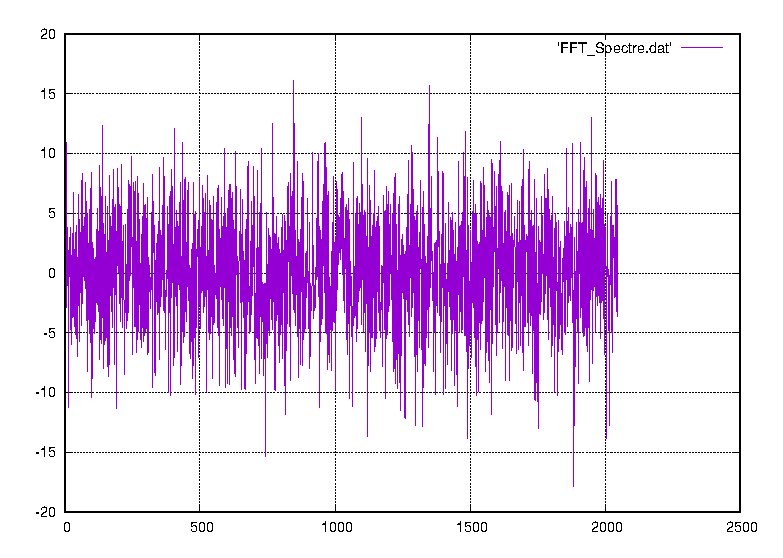
\includegraphics[height = 5.5cm]{FFT_Spectre.eps}}}
  \subfloat[][Après le moyennage]{\shadowbox{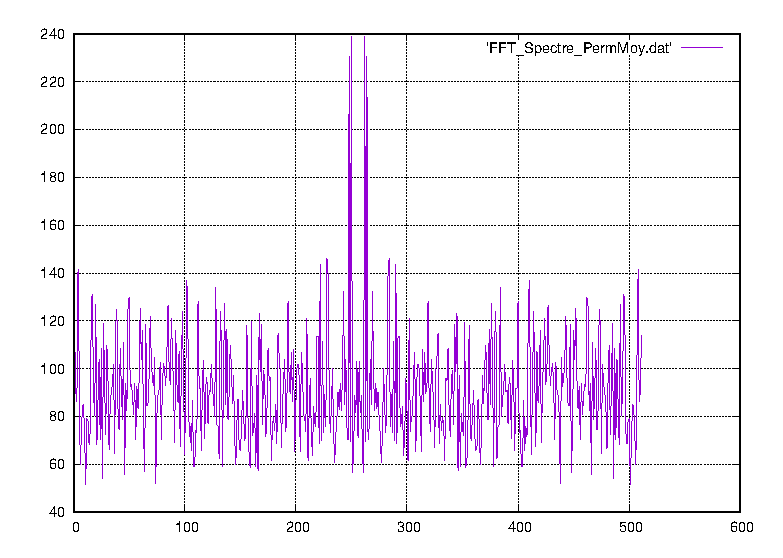
\includegraphics[height = 5.5cm]{FFT_Spectre_PermMoy.eps}}}
  \caption{TF du signal provenant de «Spectre.dat»}
\end{figure}

Le moyennage rend la détection de pic vraiment plus facile, et retire une bonne partie du bruit.

\subsection{Moyennage avec fenêtre de Hann/Hamming}
On remarque malgré l'amélioration flagrante un certain manque de définition au niveau des plus hautes fréquences. Ce manque de définition est sans doute causé par la variation importante qu'engendre le bruit dans les plus hautes fréquences. Pour éliminer ce bruit on peut moyenner les échantillons avec une fenêtre de Hann ou de Hamming pour réduire les coefficients dus au bruit et exacerber les propriétés des plus hautes fréquences.

\begin{figure}[ht!]
  \centering
  \subfloat[][Pondéré avec la fenêtre de Hamming]
           {\shadowbox{\includegraphics[height = 11.2cm]{FFT_Spectre_PermMoyHamming.eps}}}\\
  \subfloat[][Moyennage simple]
           {\shadowbox{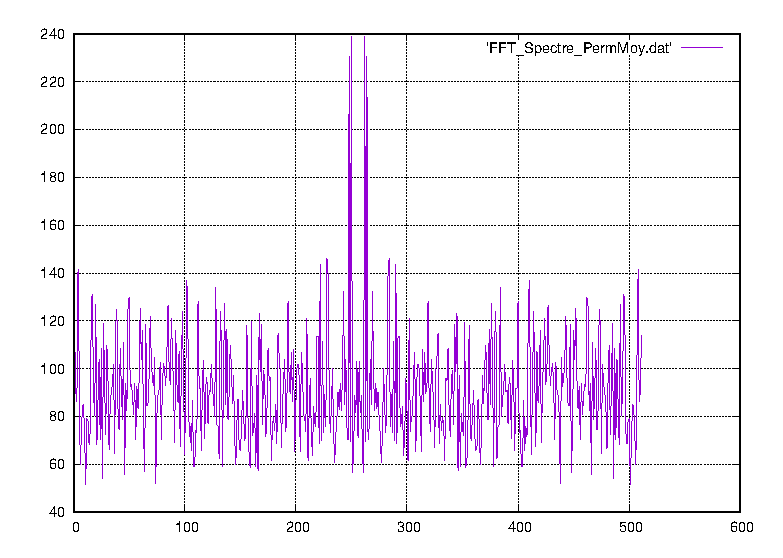
\includegraphics[height = 5.5cm]{FFT_Spectre_PermMoy.eps}}}
  \subfloat[][Pondéré avec la fenêtre de Hann]
           {\shadowbox{\includegraphics[height = 5.5cm]{FFT_Spectre_PermMoyHann.eps}}}
  \caption{TF du signal provenant de «Spectre.dat»}
\end{figure}

Comme on peut le constater d'emblée en regardant la figure 3, les graphiques pondérés par une fenêtre sont allégés au niveau du bruit. De plus, d'un point de vue analytique, ils sont bien plus utiles puisqu'il est possible de distinguer clairement de nombreux pics qui semblaient faire partie du bruit dans le graphique original.

\end{document}

